\chapter{UPPAAL Model}\label{app:UPPAAL}
In this appendix the UPPAAL model along with its code can be seen.

\begin{figure}
	\hspace{-100pt}
  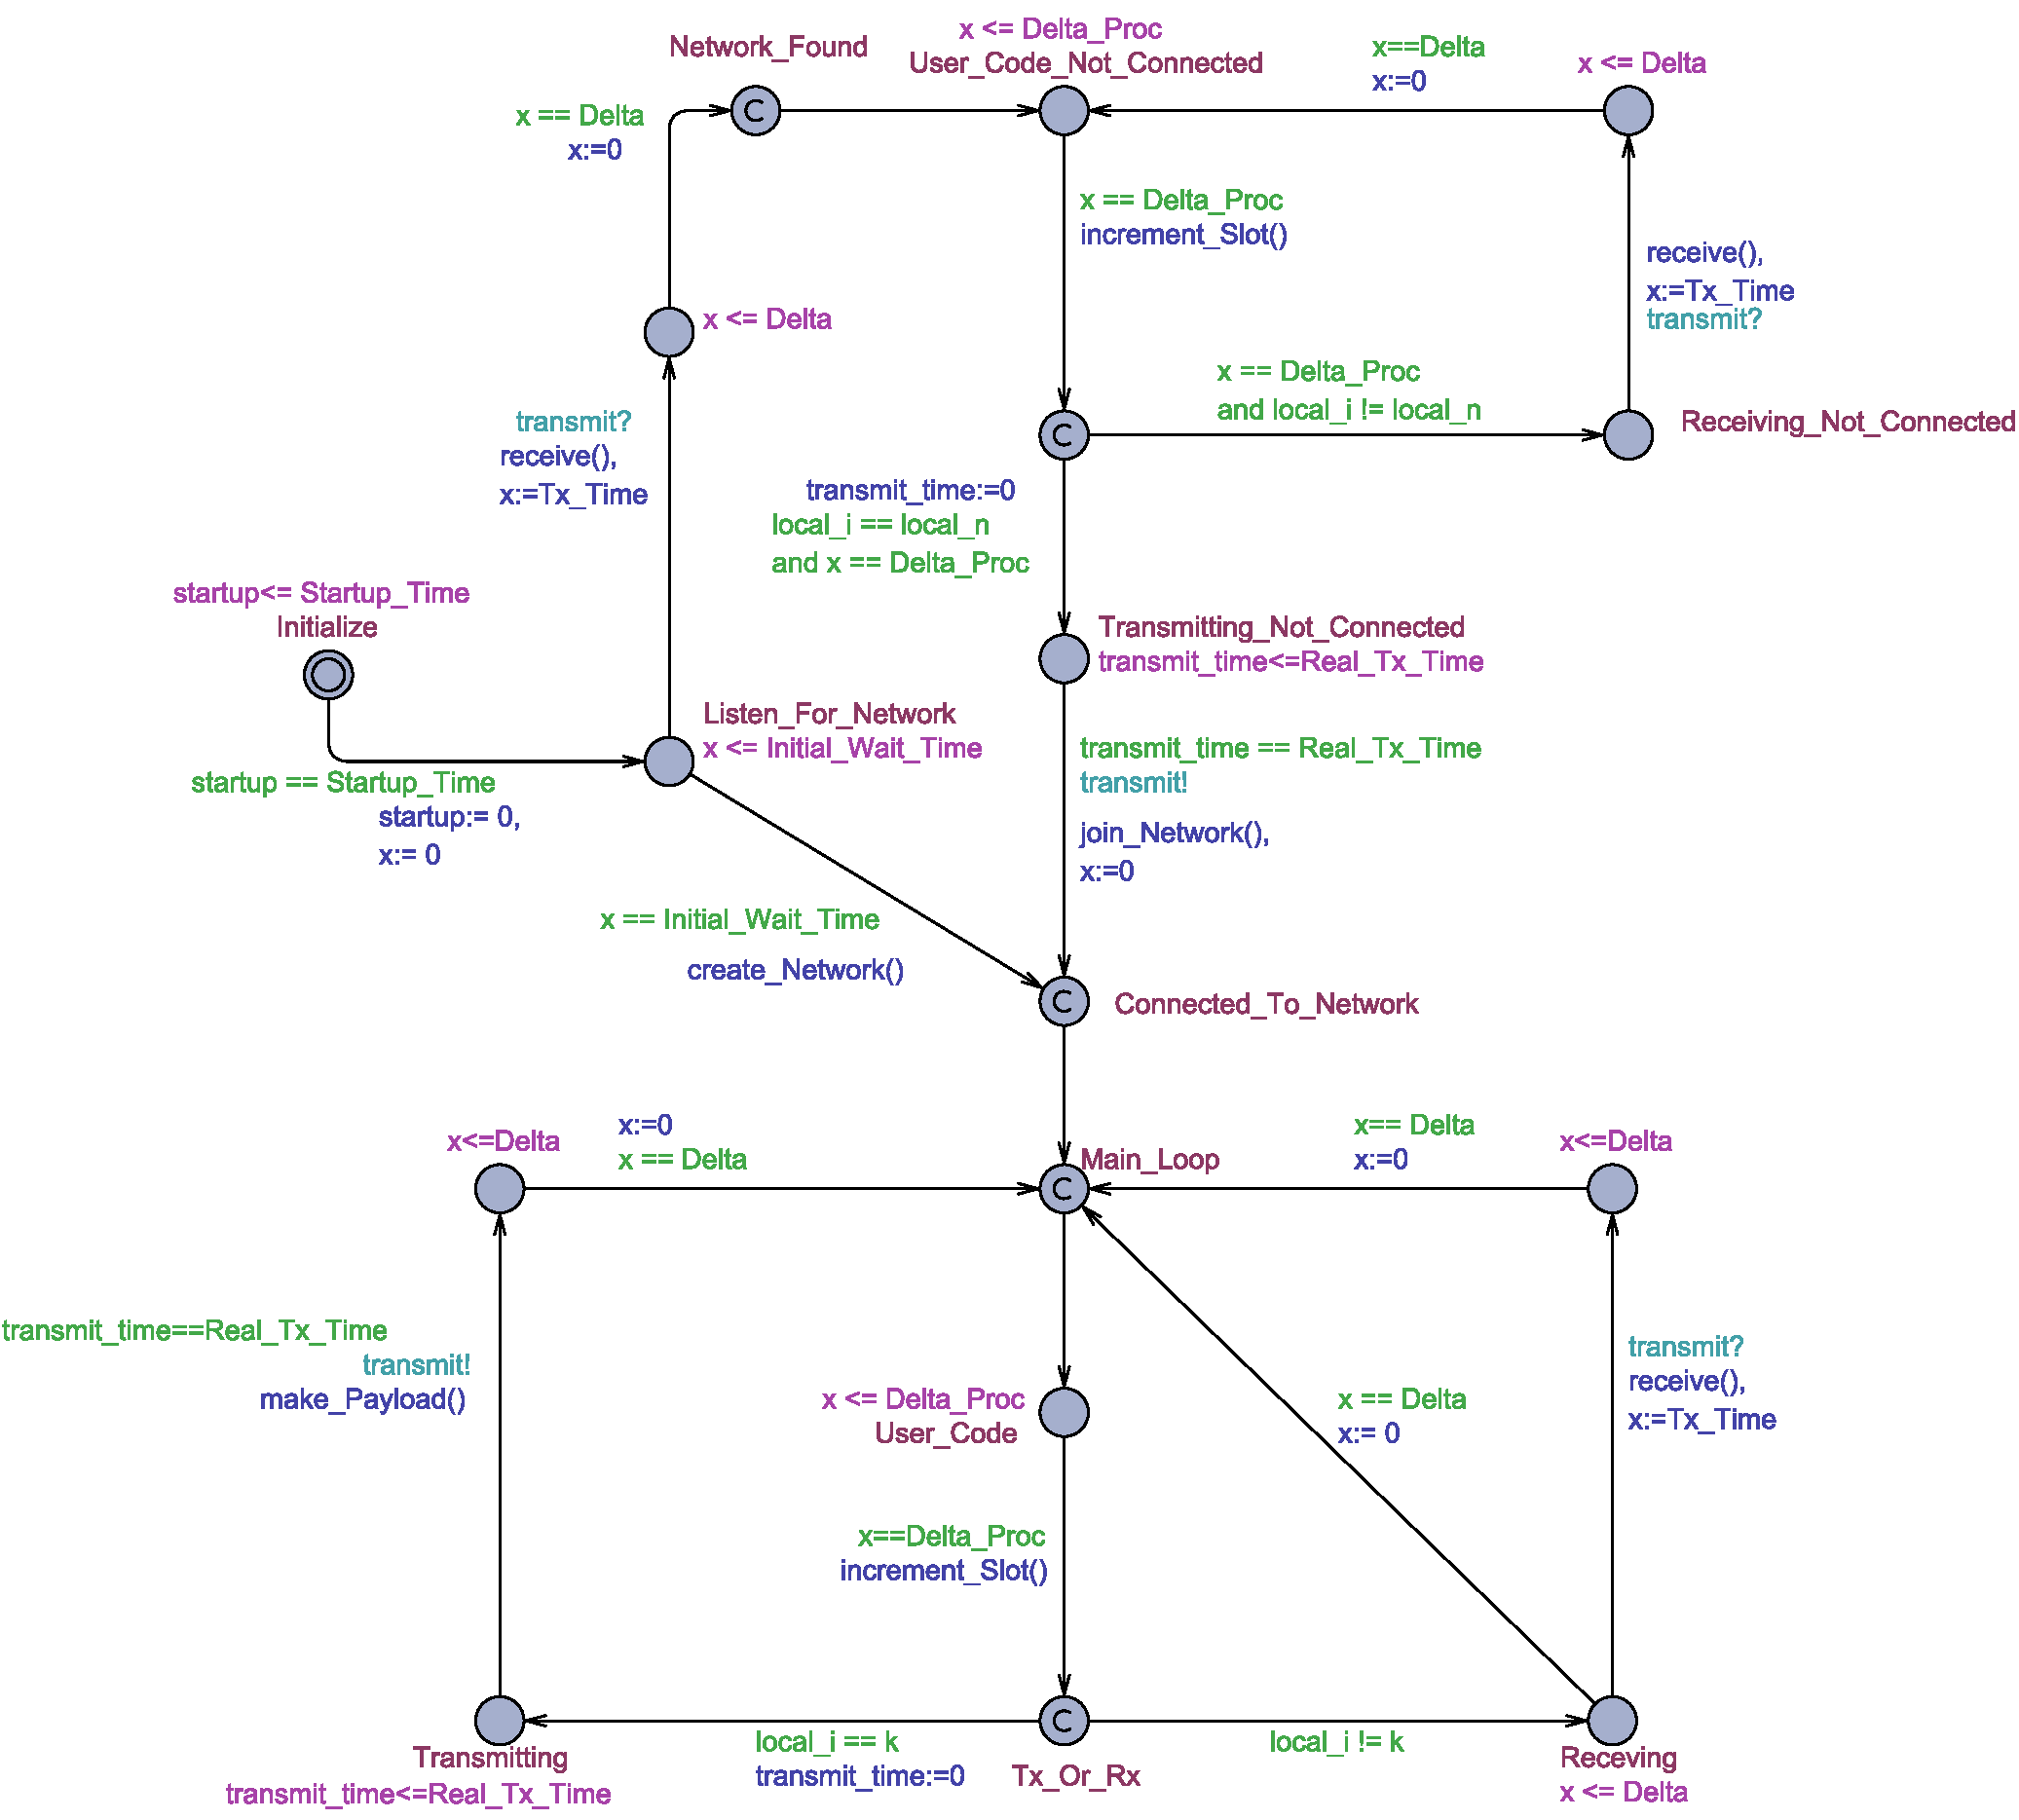
\includegraphics[width=1.40\textwidth]{Figures/Model/Device.pdf} 
\caption{UPPAAL Model}
\end{figure}

\begin{lstlisting}[language={[GUI]Uppaal}, % use GUI flavor
columns={[l]flexible},
frameround=fftt, frame=shadowbox, rulesepcolor=\color{gray},
caption={Code for the global declarations.}]
// Place global declarations here.
int n = 0;                      // Number of Timeslots connected
int i = 0;                      // Current time slot in the frame
int ConnectedCounter = 0;       //Global Counter for Connected Devices
const int Delta = 80;           //Timeslot Length
const int Delta_Proc = Delta/2;
const int Real_Transmit_Time = Delta/3;
const int Initial_Wait_Time = Delta*3;
int Startup_Time = Initial_Wait_Time*2;
clock startup;

//Channel					//Device Creation
broadcast chan transmit;	const int N = 4;
							typedef int[1,N] id_t;
\end{lstlisting}


\begin{lstlisting}[language={[GUI]Uppaal}, % use GUI flavor
columns={[l]flexible},
frameround=fftt, frame=shadowbox, rulesepcolor=\color{gray},
caption={Code for the local declarations for Device.}]
// Place local declarations here.
clock x;
clock transmit_time;
int k = -1;                     //Timeslot
bool Connected = false;

// Local copies of globals
int local_n = 0;                // Number of devices connected
int local_i = 0;               // Current time slot in the frame

void increment_Slot(){					void receive(){
local_i = (local_i % local_n)+1;		  	local_i = i;
}										  	local_n = n;
										}

void join_Network(){					void create_Network(){
k=n;									  	i = 1;
i = 1;										n = 2;
local_i = 1;								k = 1;
n = n+1;									local_i = 1;
local_n = local_n+1;						local_n = 2;
}										}

void make_Payload(){
i = local_i;
n = local_n;
}
\end{lstlisting}

\begin{lstlisting}[language={[GUI]Uppaal}, % use GUI flavor
columns={[l]flexible},
frameround=fftt, frame=shadowbox, rulesepcolor=\color{gray},
caption={Code for system declarations.}]
// Place template instantiations here.
// List one or more processes to be composed into a system.
system Device;
\end{lstlisting}